 %%%%%%%%%%%%%%%%%%%%%%%%%%%%%%%%%%%%%%%%%%%%%%%%%%%%%%%%%%%%%%%%%%%%%%%%%%%%%%%%%%%%%
% ITR_LSR_slides class options
% - 'itr' or 'ITR' for ITR version
% - 'lsr' or 'LSR' for LSR version
% - 'german' for a German presentation
% - 'english' for an English presentation (default)
% - 'longpres' if you want to use subsections
% - 'noshadow' if you want to use blocks without shadow
% - 'draftlayout' to show a mm grid as overlay for precise positioning
% - 'presentermode' to generate slides with note-page, usable with e.g. pympress
% - 'coveredhidden' to hide covered objects. Default is transparent.
% beameroptions can be used, e.g.:
% - 'aspectratio=169' for 16:9 wide screen presentations
% - `handout` to generate printable handout sheets
% - `draft` for fast compilation (without graphics)
% do not remove STUDENT option!
%%%%%%%%%%%%%%%%%%%%%%%%%%%%%%%%%%%%%%%%%%%%%%%%%%%%%%%%%%%%%%%%%%%%%%%%%%%%%%%%%%%%%
\documentclass[student, noshadow, lsr, english, aspectratio=169]{ITR_LSR_slides}
\usepackage{tikz}
\usepackage{pgfplots}
\pgfdeclarelayer{background}
\pgfdeclarelayer{nodelayer}
\pgfdeclarelayer{edgelayer}
\pgfdeclarelayer{foreground}
\pgfsetlayers{background,edgelayer,nodelayer,main,foreground}
% robot name for tikz figure
%\newcommand{\RobotName}{$\mathbf{R}$}

\def\CheckAttentionSlide{
    \begin{frame}
        \begin{center}
            {\fontsize{40}{50} \structure{Sorry for your attention}\\}
        \end{center}
    \end{frame}
}

\addbibresource{./refs/mybib.bib}
\graphicspath{{pics/}{logos/}}

\title{Kernel Embedding for Particle Gibbs-Based Optimal Control}
\presenter{L. Hochschwarzer}

\supervisor{R. Lefringhausen}
\typeofpres{Intermediate Report Master‘s Thesis}

\usepackage[bigfiles]{media9} %option bigfiles not needed for xelatex, runs without problems on ubuntu14
%%%%%%%%%%%%%%%%%%%%%%%%%%%%%%%%%%%%%%%%%%%%%%%%%%%%%%%%%%%%%%%%%%%%%%%%%%%%%%%%

\usepackage{empheq}

\begin{document}


\begin{frame}
    \titlepage
\end{frame}


\section{Introduction}
\begin{frame}{Motivation}	
...
\end{frame}


\begin{frame}{Related Works}
Particle Markov Chain	
\cite{Robert_24}, \cite{Andrieu_10}

Kernel Embeddings:
\cite{Yassine_22}

\end{frame}


\begin{frame}{Problem Statement}	
...
\end{frame}


\section{Particle Gibbs}

\begin{frame}{Particle Markov Chain Monte Carlo}
...
\end{frame}

\begin{frame}{Particle Markov Chain Monte Carlo - Samples}
...
\end{frame}

\begin{frame}{Scenario Generation}
...
\end{frame}


\section{Kernel Embedding}

\begin{frame}
	\frametitle{MMD ambiguity sets}
	
\end{frame}

\begin{frame}
	\frametitle{Constraint Reformulation}
\textbf{Goal:} Reformulate chance-constraint problem with $\boldsymbol{\delta}^{[1:N]}$
\begin{block}{Feasible Region of chance constraint}
\begin{equation*}
Z_i :=  \left\{ \boldsymbol{u}_{0:H} \in \mathcal{U}^{H+1} : \inf\limits_{P \in \mathcal{P}}P \left[ \tilde{h}_i(\boldsymbol{u}_{0:H},  \boldsymbol{\delta}) \leq 0 \right] \geq 1 - \alpha \right\}
\end{equation*}
\end{block}	

\makebox[6.7cm]{\hfill} $\boldsymbol{\Downarrow}$ 

\begin{block}{Reformulated Feasible Region}
\begin{empheq}[right = \empheqrbrace, left= Z_i \coloneqq \empheqlbrace \boldsymbol{u}_{0:H} \in \mathcal{U}^{H+1} :]{align*}
    & g_0 + \frac{1}{N}\sum_{n = 1}^N (\boldsymbol{K}\boldsymbol{\gamma})_n + \varepsilon \sqrt{\boldsymbol{\gamma}^\text{T}\boldsymbol{K}\boldsymbol{\gamma}} \leq t \alpha \\
    & [\tilde{h}_i(\boldsymbol{u}_{0:H},  \boldsymbol{\delta}^{[n]}) + t]_+ \leq g_0 + (\boldsymbol{K}\boldsymbol{\gamma})_n, \; n = 0,...,N \\
    & g_0 \in \mathbb{R}, \boldsymbol{\gamma} \in \mathbb{R}^N, t \in \mathbb{R}
  \end{empheq}
\end{block}
\end{frame}


\begin{frame}
	\frametitle{Problem Formulation}
\textbf{Goal:} Reformulate chance-constraint problem with $\boldsymbol{\delta}^{[1:N]}$ \\
\begin{align*} 
 &\min\limits_{\boldsymbol{u}_{0:H}, \overline{J_H}}  \overline{J_H}\\
\text{subject to:}&\; \forall n \in \mathbb{N}_{\leq N}, \;  \forall \in \mathbb{N}_{\leq H}^0  \\
&\left. 
\begin {aligned}
\boldsymbol{x}_{t+1}^{[n]} = \boldsymbol{f}_{\boldsymbol{\theta}^{[n]}} \left( \boldsymbol{x}_{t}^{[n]} , \boldsymbol{u}_t \right) + & \boldsymbol{v}_{t}^{[n]} \\
\boldsymbol{y}_{t} = \boldsymbol{g}_{\boldsymbol{\theta}^{[n]}} \left( \boldsymbol{x}_{t}^{[n]}, \boldsymbol{u}_t \right) + & \boldsymbol{w}_{t}^{[n]}
\end{aligned}
 \;\;\; \right\} \; \text{Dynamic Constraints} \\
&\;\;\;\; J_H(\boldsymbol{u}_{0:H},  \boldsymbol{x}_{0:H}^{[n]},  \boldsymbol{y}_{0:H}^{[n]})  \leq \overline{J_H} \\
&\;\;\;\; \boldsymbol{u}_{0:H} \in Z_i, \forall i = 1, ...,n_c \;\;\;\;\;\;\;\;\; \Bigl\} \; \text{Reformulated Chance Constraints}
\end{align*}



\end{frame}

\section{Simulation}

\begin{frame}{Simulation Setup (1/2)}
\begin{itemize}
\item 
\makebox[4cm]{Unknown system: \hfill}
$\boldsymbol{f}(\boldsymbol{x}, u) = 
\begin{bmatrix}
0.8  x_1 - 0.5 x_2 \\
0.4 x_1 + 0.5 x_2 + u
\end{bmatrix}$ \\
\makebox[4cm]{\hfill} $\boldsymbol{v}_t \sim \mathcal{N} \left(\boldsymbol{0}, \boldsymbol{Q} =  
\begin{bmatrix}
0.03 & \text{-}0.004 \\
\text{-}0.004 & 0.01
\end{bmatrix}
\right).$

\item Known observation function $g(\boldsymbol{x}, u) = x_1$ and measurement noise $w_t \sim \mathcal{N} (0, 0.1)$

\item Known initial state $\boldsymbol{x}_{\text{-}T} \sim \mathcal{N} ([2, 2]^\text{T}, \boldsymbol{I}_2)$ 

\item Known input/output measurements $\mathbb{D} = \left\{\boldsymbol{u}_{t}, \boldsymbol{y}_{t}\right\}_{t = \text{-}T:\text{-}1}$

\item Cost function $J_H = \sum_{t = 0}^H u_t^2$

\item Input constraints $\left| u \right| \leq 10$

\item Output constraints $y_{10:20} \leq (\text{-} 10)$ and $10 \leq y_{30:40}$
\end{itemize}
\end{frame}

\begin{frame}{Simulation Setup (2/2)}
Particle Marcov chain Monte Carlo \cite{Svensson_17}:
\begin{itemize}
\item Known basis functions $\boldsymbol{\varphi}(\boldsymbol{x}_t, u_t) =  \left[ x_1,  x_2,  u \right]^\text{T}$ \\
	$\Rightarrow \boldsymbol{f}(\boldsymbol{x}, u) = \boldsymbol{A} \boldsymbol{\varphi}(\boldsymbol{x}_t, u_t) + \boldsymbol{v}_{t}, \; \boldsymbol{v}_{t} \sim \mathcal{N} (\boldsymbol{0}, \boldsymbol{Q}), \; \boldsymbol{\theta} = \{\boldsymbol{A}, \boldsymbol{Q}\}$

\item
\makebox[3cm]{Priors: \hfill} $\boldsymbol{Q} \sim \mathcal{IW} (100 \boldsymbol{I}_2, 10)$ 
\makebox[3cm]{\hfill} $\boldsymbol{A} \sim \mathcal{MN} (\boldsymbol{0}, \boldsymbol{Q}, 10 \boldsymbol{I}_2)$ 
\item $N_p = 1000,\; n_d = 30$
\end{itemize}
Kernel Embedding:
\begin{itemize}
\item Gaussian kernels $k(x,y) = \text{exp}\left(\text{-}\frac{1}{2\sigma^2} ||x - y||_2^2 \right)$ for all 4 random varibles
\item Bandwidth $\sigma$ set via the median heuristic \cite{Damien_18} and scaled with factors $\left[ 1.5, 5, 5, 1 \right]^\text{T}$
\end{itemize}
\end{frame}	

\begin{frame}{Optimal Control with Constrained Outputs}

Number of scenarios used for optimization: $N = 200$
\vspace{.3cm}
\begin{columns}[onlytextwidth, T]
		\begin{column}{.5\textwidth}
			\;\; Scenario Approach
			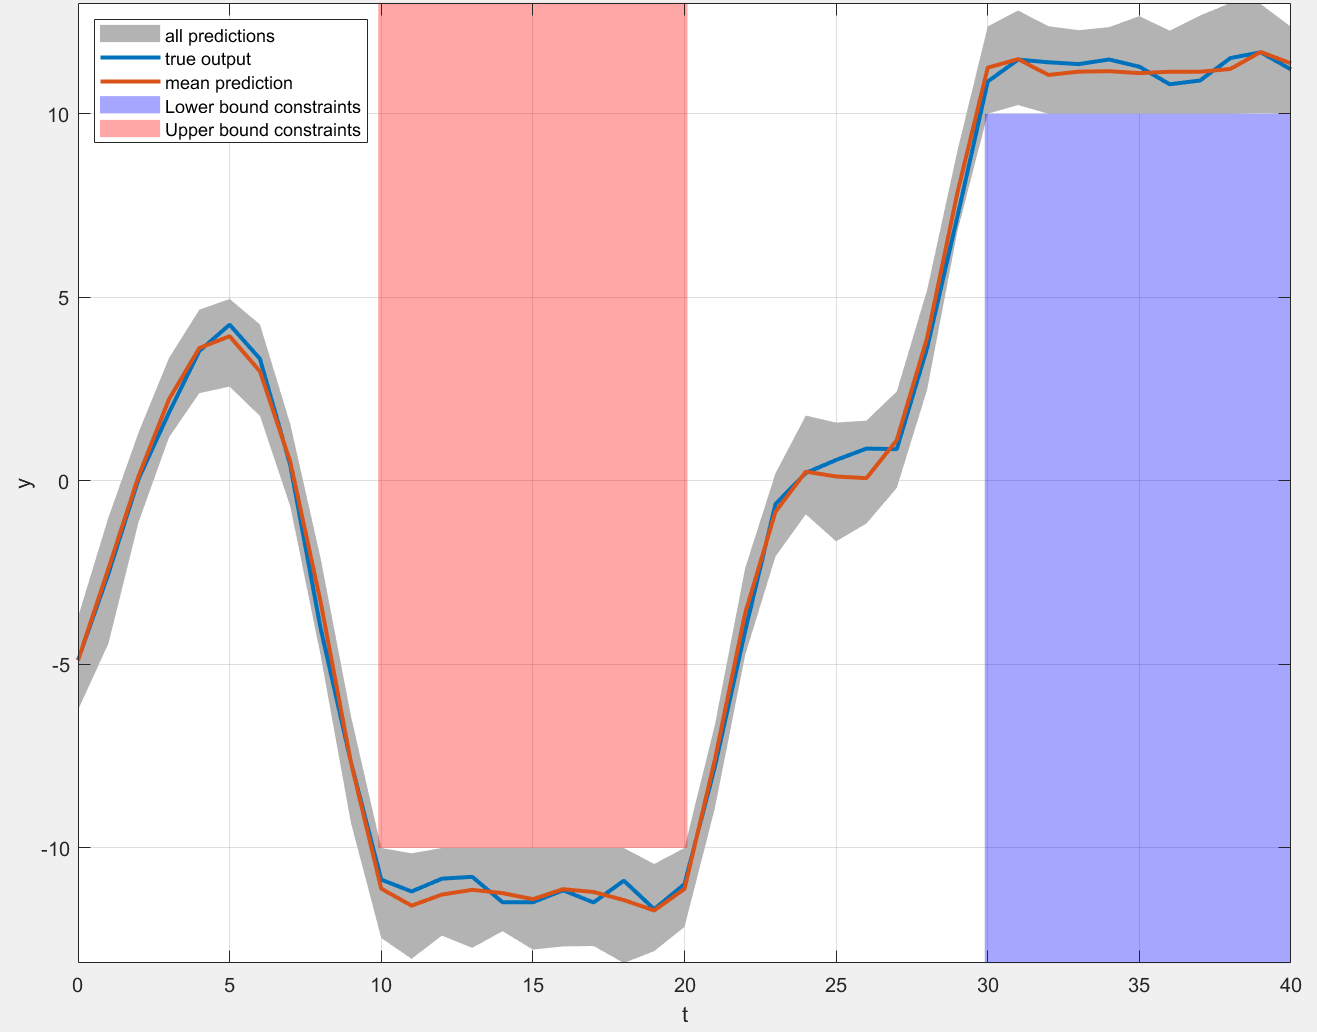
\includegraphics[width= .9\textwidth]{Scenario_plot}
		\end{column}
		\begin{column}{.5\textwidth}
			$\;\;$ Kernel Approach  ($\alpha = 0.1$)
			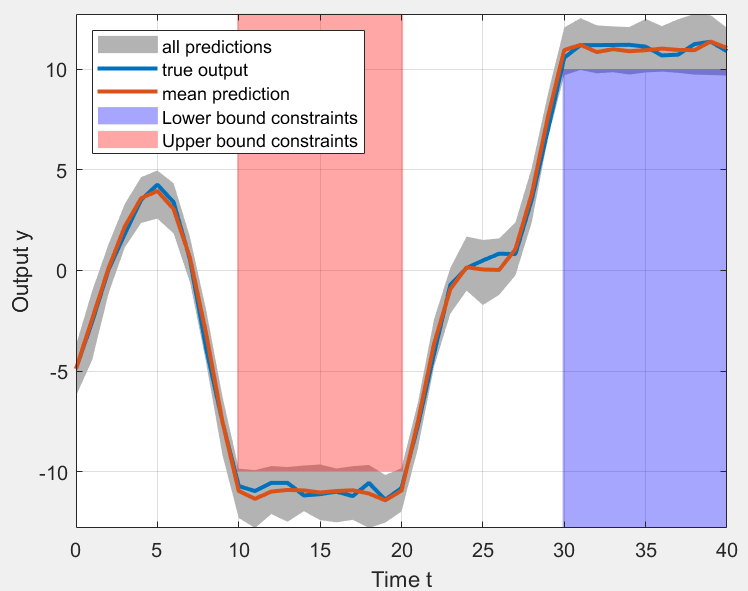
\includegraphics[width=.9\textwidth]{Kernel_plot}
		\end{column}
	\end{columns}\vspace{.5cm}
\end{frame}	

\begin{frame}{Successrate of Solution}
	\vspace{.2cm}
	\begin{columns}[onlytextwidth, T]
		\begin{column}{.5\textwidth}
			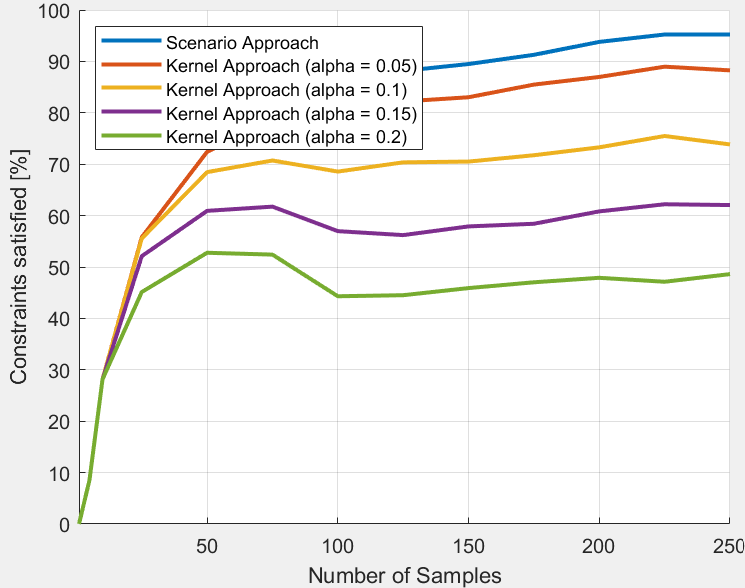
\includegraphics[width=.9\textwidth]{robustness_plot}
		\end{column}
		\begin{column}{.5\textwidth}
			xAxis: Number of scenarios used to find the solution $u_{0:H}$ \\
			\vspace{.1cm}yAxis: Percentage of scenarios where $u_{0:H}$ satisfies the output constraints \\
			\vspace{.4cm}$N = 2000$ Number of Scenarios used to test $u_{0:H}$
		\end{column}
	\end{columns}\vspace{.5cm}
\end{frame}	

\begin{frame}{Computation Time}
\vspace{.2cm}
\begin{columns}[onlytextwidth, T]
		\begin{column}{.5\textwidth}
			\vspace{.4cm}
			xAxis: Number of scenarios used to formulate OCP \\
			\vspace{.2cm}yAxis: Time to find solution $u_{u:H}$ \\
		\end{column}
		\begin{column}{.5\textwidth}
			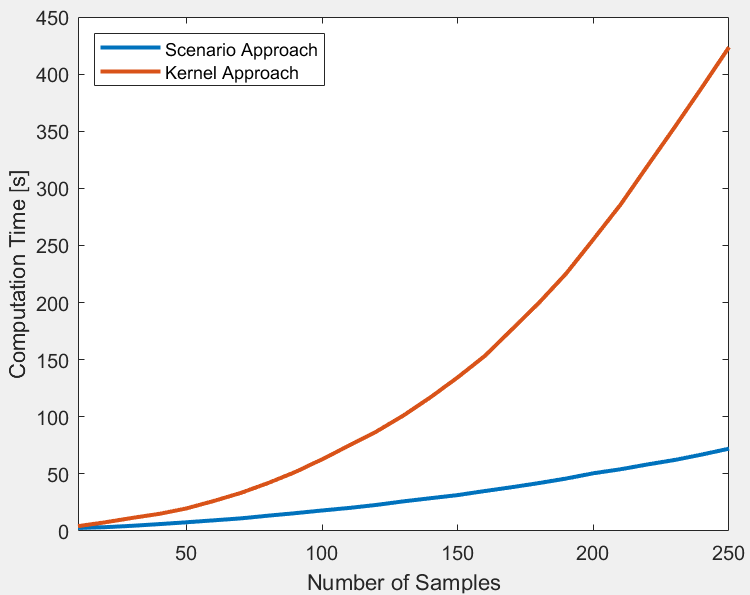
\includegraphics[width=\textwidth]{/computationtime_plot}
		\end{column}
	\end{columns}\vspace{.5cm}
\end{frame}	

\section{Conclusion}

\begin{frame}{Summary}
	...
\end{frame}

\begin{frame}{Future Plans}
	\begin{itemize}
	\item Parameter tuning of $\sigma$
	\item Risk factor for all constraints at once instead of individually
	\item Use Kernel Embeddings on non-linear systems
	\end{itemize}
\end{frame}

	\appendix
	% This slide serves 3 purposes:
	% 	1. a simple example how to create figures in tikz using beamer
	%	2. testing if you actually checked the content of this template
	% 	3. subtly preventing you from adding a "Thank you..." slide at the end of your presentation
	% If this slide is still in your final presentation... well, congratulation!
	\CheckAttentionSlide


%\nocite{buss11}
%\nocite{bauer09}
\begin{frame}{\LSRITRRefTitle}
	\printbibliography
\end{frame}


\end{document}
